\chapter{Implementation}
The chapter will explain how the different software are connected and what information is sent between them. All the configuration and start up commands can be found in the appendix.
\section{Software implementation}
The software implementation consist mainly of rtklib and dune. Piksi is also used in the experiment, however it's rtklib and the Dune task RTKGPS that will be discussed thoroughly.
\subsection{Rtkgps}
The structure of rtkgps which will include the rtkgps task in dune, the connection to rtklib the piksi task in dune, the output message.

Rtklib is separated into the base station and the rover. The base station implementation runs the app str2str were it communicate with the ublox over a uart cable, and start up a tcp server.

The rover uses the rtkrcv app from rtklib to estimate the position of the rover. Rtkrcv connect itself as a tcp client to the tcp server that str2str create. Rtkrcv is configured in a moving baseline configuration to simulate the behavior that is expected during a landing on a ship. (Referer her til teori kap om rtklib)

Rtkrcv output the solution data over a virtual uart connection that is created by a program called socat. The output structure is given i (se rtklib com kap)

Rtkgps is a task in Dune that takes the output from rtklib and create a rtkfix imc message that is dispatch into the Dune/Neptus network. Rtkgps consists of two parts. One reads the message from the virtual uart, and the other create and dispatch the rtkfix imc message.
\begin{table}[!h]
\begin{center}
    \begin{tabular}{ | l | l |}
    \hline
    \textbf{Header} & \textbf{Content} \\ \hline
     tow & Gps time of Week  \\ \hline
     n & Baseline North coordinate \\ \hline
     e & Baseline East coordinate \\ \hline
     d & Baseline Down coordinate \\ \hline
     v\verb=_=n & Velocity North coordinate \\ \hline
     v\verb=_=e & Velocity East coordinate \\ \hline
     v\verb=_=d & Velocity Down coordinate \\ \hline
     iar\verb=_=hyp & Number of hypotheses in the Integer Ambiguity Resolution \\ \hline
     iar\verb=_=ratio & Quality ratio of Integer Ambiguity Resolution \\ \hline
     type & Type of fix: \\& None = No solution, but RTK task is running
     \\& Obs = No solution, but receiving observations
     \\& Float = Floating point solution of Integer Ambiguity Resolution
     \\& Fix = Fixed(single) solution of Integer Ambiguity Resolution \\ \hline
    \end{tabular}
\end{center}
\caption{The \gls{imc} message RtkFix }
\label{Tb:RtkFix}
\end{table}

\section{Hardware implementation}
The embedded computer uses GLUED as its operating system, and on it runs both Dune and rtklib. The Piksi and Ublox is connected to the BeagleBone over uart cables.

Has a WIFI connection to the base station.
TRENGER SYSTEM FIGUR SOM VISER HVORDAN UAV ER FORBUNDET MED BASE
The two \gls{rtk-gps} system is connected to a antenna splitter , figure \ref{figure:AntennaSplitter}, such that both system receive the same \gls{gnss} signals.

\begin{figure}[H]
	\centering
		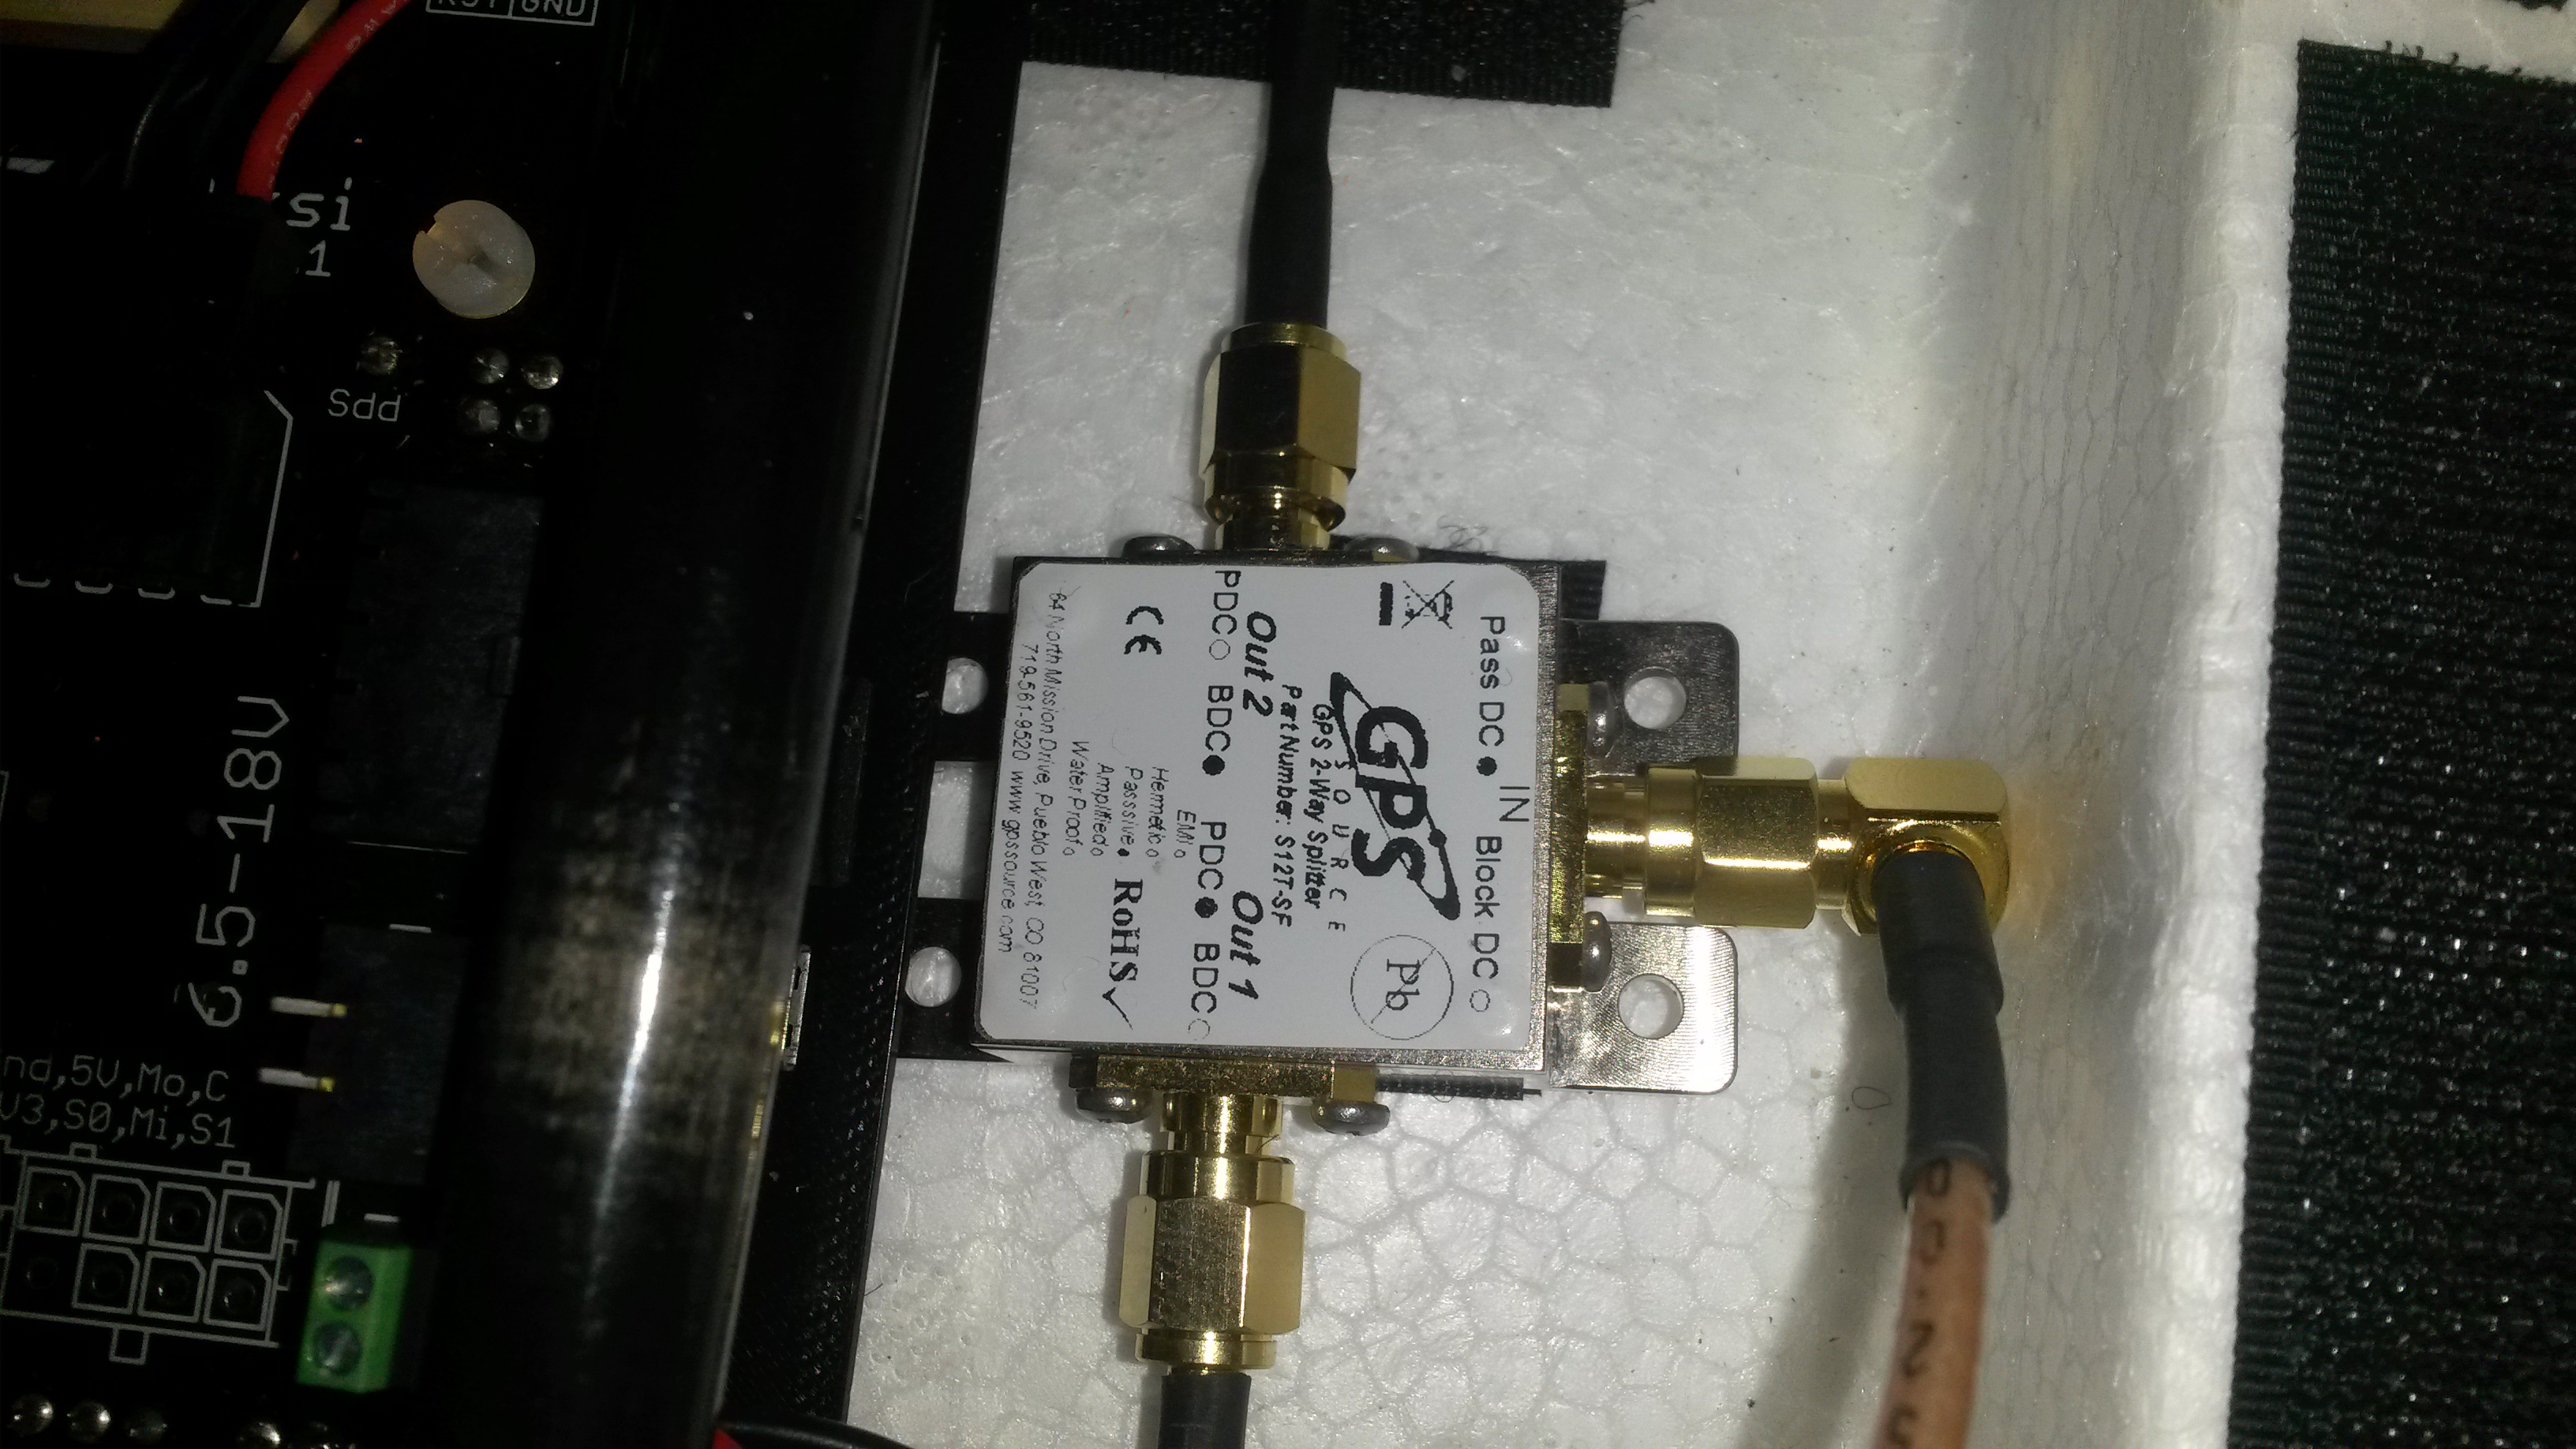
\includegraphics[width=0.7\textwidth]{figs/066.jpg}
		\caption{Antenna splitter}
		\label{figure:AntennaSplitter}
\end{figure}

This section contain how all the physical components are connected at both the rover and the base station. Include also how everything was prepared.

About Beaglebone: What runs on the beaglebone, connections, devices, what is it place in the system

About Ublox: Explain the ublox from a system perspective, how it's connected

Pixhawk: What do it do in the system:

Piksi: Same as ublox

The X8: How do it fit in the system

The base station: Same as x8

Antennas: 

Wifi router

